% IEEE standard conference template; to be used with:
%   spconf.sty  - LaTeX style file, and
%   IEEEbib.bst - IEEE bibliography style file.
% --------------------------------------------------------------------------

\documentclass[letterpaper]{article}
\usepackage{spconf,amsmath,amssymb,graphicx,bm,xcolor,listings}

% Example definitions.
% --------------------
% nice symbols for real and complex numbers
\newcommand{\R}[0]{\mathbb{R}}
\newcommand{\C}[0]{\mathbb{C}}
\newcommand{\N}[0]{\mathbb{N}}

% bold paragraph titles
\newcommand{\mypar}[1]{{\bf #1.}}

% inline
\newcommand{\inline}[1]{{\ttfamily\hyphenchar\font=45 #1}}

% listings style for c++ code
\lstdefinestyle{cppstyle}{
  language=C++,
  basicstyle=\small\ttfamily,
  keywordstyle=\color{blue},
  commentstyle=\color{green!60!black},
  stringstyle=\color{red},
  showstringspaces=false,
  breaklines=true,
  breakatwhitespace=true,
  tabsize=4,
  numbers=left,
  numbersep=5pt,
}

% Title.
% ------
\title{High-Performance Implementation Strategies for Texture Synthesis}
%
% Single address.
% ---------------
\name{Tal Rastopchin \qquad  Svitlana Morkva \qquad  Ivan Sobko \qquad  Baptiste Goumain}
\address{Department of Computer Science\\ ETH Zurich, Switzerland}


\begin{document}

% Add page numbers
\pagestyle{plain}
\pagenumbering{arabic}

%\ninept
%
\maketitle
%

\begin{abstract}
Describe in concise words what you do, why you do it (not necessarily
in this order), and the main result. The abstract has to be
self-contained and readable for a person in the general area. You
should write the abstract last.
\end{abstract}

\section{Introduction}\label{sec:intro}

Image quilting algorithms have become indispensable tools in various image processing applications, providing solutions for texture synthesis, seamless image stitching, and image inpainting. However, with the ever-increasing demand for real-time performance and the handling of large-scale textures, there is a growing need for high-performance versions of image quilting algorithms that can efficiently and effectively process images, while maintaining visual quality. The objective of this paper is to introduce and evaluate a high-performance version of the image quilting algorithm that addresses the computational challenges and improves overall efficiency. 

\mypar{Motivation} The motivation behind this research arises from the limitations of traditional image quilting algorithms in meeting the demands of modern applications. Standard approaches often struggle to handle high-resolution images hindering their usability in areas such as video games, virtual reality, and live video processing. Additionally, the computational complexity associated with large-scale textures poses challenges in terms of memory consumption and processing time. Therefore, a high-performance version of the image quilting algorithm is crucial to overcome these limitations and unlock its full potential in various domains.

\mypar{Contribution}
In this study, we present an optimized implementation of the image quilting algorithm, focusing on key areas such as enhancements to a straightforward algorithm, loop unrolling, block processing and SIMD vectorization. We explore innovative approaches that leverage modern hardware architectures, including Central Processing Units (CPUs), to accelerate the algorithm's execution time. By harnessing the knowledge of modern CPU's execution units, we aim to significantly improve the overall performance of the algorithm while maintaining the quality of generated textures

\mypar{Related work} \textbf{TODO}: Next, you have to give a brief overview of
related work. For a paper like this, anywhere between 2 and 8
references. Briefly explain what they do. In the end contrast to what
you do to make now precisely clear what your contribution is.


\section{Background on Image Quilting}\label{sec:background}

Within this section, our objective is to present a formal definition of Image Quilting, introduce the essential components of the algorithm alongside our implementation, conduct a cost analysis, and outline the asymptotic complexity of the problem.

\mypar{Image Quilting}
Texture synthesis refers to the process of generating new, realistic textures based on a given input texture or a set of exemplar textures. The goal is to create a larger texture that captures the visual characteristics and patterns present in the input textures.
Image Quilting is a common approach of patch-based synthesis, where small patches of the input texture are used to iteratively reconstruct the larger texture. These patches are selected based on their similarity to the surrounding context, ensuring that they fit seamlessly into the overall texture. The algorithm consists of three key components that progressively enhance both the algorithm itself and the resulting output texture.

We can define \textit{$B_{i}$} as a synthesis unit, which is a square block of user-specified size extracted from the set \textit{$S_{B}$} containing all overlapping blocks in the input texture image. The most straightforward approach to generating a larger texture involves randomly sampling blocks from \textit{$S_{B}$}. Although this method produces textures of the desired size, they exhibit noticeable flaws due to the lack of correspondence between selected blocks, resulting in clearly visible seams.

To address this imperfection, a solution is to randomly sample only the top-left corner block. For all other positions, we would search for a block in \textit{$S_{B}$} that agrees with its neighboring blocks in the output texture. The agreement between the chosen \textit{$B_{i}$} from \textit{$S_{B}$} and its neighboring blocks is typically evaluated using the $\ell ^2$-norm function on the overlap regions. In the Image Quilting algorithm, the overlap region is commonly defined as one-sixth of the block size, with the blocks stitched in the middle of this overlap region. The error tolerance was set to be within 0.1 times the error of the best matching block. The stitching process can be categorized into three separate cases: vertical stitching for the first row, horizontal stitching for the first column, and corner stitching for all other blocks.

While the previous approach has significantly improved the output, there are still instances where the seams remain noticeable. This is because the blocks are stitched together using straight lines, which can be easily detected by the human eye. Therefore, in the next component of the algorithm, we aim to further reduce this problem by identifying a minimum cost path through the error surface within the overlap region. To perform the Minimum Error Boundary Cut using dynamic programming, we define the error surface as ${e = (B^{ov}_{1} - B^{ov}_{2})^{2}}$, where ${B^{ov}_{1}}$ and ${B^{ov}_{2}}$ represent the overlap regions of two blocks. The goal is to compute the cumulative minimum error, E, for all possible paths as:
\[ E = e_{i,j} + min(E_{i-1,j-1}, E_{i-1,j}, E_{i-1,j+1}). \]
The minimum value in the last row of the table represents the end of the best stitching path. To obtain the whole path, we traverse back from this minimum value, selecting the cells with the minimum cumulative error at each step until we reach the first row.

\mypar{Cost Analysis} Our definition of the cost measure is informed by our initial profiling of our baseline implementation. In particular, generating a flame graph (made using CLion's DTtrace-based CPU profiler on MacOS) revealed that about 85\% of the runtime of the algorithm was devoted to computing the $\ell ^2$-norm between block overlap regions. About only 3\% of the runtime was devoted to computing the minimum cut and writing the block. Because the computation of the $\ell ^2$-norm dominates the runtime of the algorithm, we decided to define our cost measure in terms of the operations required to compute the $\ell ^2$-norm.

Because the input to our algorithm is an image, which are most commonly encoded as two-dimensional arrays of packed 1-byte wide red, green, blue, and alpha channels, we decided to focus our implementation and cost measure on integer operations. CPUs are designed to have many more integer ALUs than Floating Point execution units because integer arithmetic is much more common than floating point arithmetic. Furthermore, using the narrowest numeric type appropriate would allow higher performance when applying applying SIMD intrinsics.

To define our cost measure let's derive the number of operations needed to compute the $\ell ^2$-norm between two pixels. Let's assume that each pixel $\bm{p}_i$ has 4 channels, namely the RGBA channels. We then have that
\begin{align*}
  |\bm{p}_i - \bm{p}_j| ^2 & = (r_i - r_j)^2 + (g_i - g_j)^2 \\
  & + (b_i - b_j)^2 + (a_i - a_j)^2.
\end{align*}
We would lastly take the square root, but because we are interested in the minimum among all $\ell ^2$-norms, we can find the minimum squared $\ell ^2$-norm and get rid of the square root entirely. For $n$ pixels we can then define the following integer cost measure:
\[
  C(n) = C _\text{int add / sub} \cdot N _\text{int add / sub} + C_\text{int mul} \cdot N _\text{int mul}.
\]
We have $4n$ subtractions, $3n$ additions, $4n$ multiplications, and $n-1$ additions from adding the resulting squared $\ell ^2$-norms together. This means our cost measure is
\[
  C(n) = C _\text{int add / sub} \cdot (8n - 1) + C_\text{int mul} \cdot 4n.
\]

It is important to note that addition and subtraction usually have smaller latency and gap than multiplication. According to Agner Fog's Instruction tables, we have that for the Intel Skylake microarchitecture, the Add, Sub, and Mul integer instructions have the following latencies and throughputs:

\begin{center}
  \begin{tabular}{c|c|c}
    & Latency & Throughput \\
    \hline
    Add, Sub & 1 cycle & 4 per cycle \\
    \hline
    Mul & 3-4 cycles & 1 per cycle \\
  \end{tabular}
\end{center}

This means that the cost of an integer multiplication is greater than the cost of an integer addition or subtraction.

An asymptotic analysis of the image quilting algorithm further justifies our choice of cost measure. The original image quilting paper \cite{Efros:01} does not perform an asymptotic analysis and so we provide one here. For the purpose of the asymptotic analysis, assume that the input image is square and has $n \in \N$ pixels. Then, it has a width and height of $I_w = I_h := \sqrt{n} \in \N$ pixels. Further assume that the output image is also square and linearly proportional to the dimensions of the input image. Then, the ouput image has a width and height of $O_w = O_h := a \sqrt{n} \in \N$ pixels (for some valid $a \ge 1$ with $a \in \R$). Further assume that the blocks are square and their dimensions are linearly proportional to the dimensions of the input image. Then, the block size has a width and height of $B_w = B_h := b \sqrt{n} \in \N$ pixels (for some valid $0 < b < 1$ with $b \in \R$). Each block then consists of $b^2 n \in \N$ pixels.

The image quilting algorithm will then need to select
\[
  \frac{O_h}{B_h} \cdot \frac{O_w}{B_w} = \frac{(a \sqrt{n})^2}{(b \sqrt{n})^2} = \frac{a^2}{b^2} = c_0 \; \text{blocks},
\]
for some constant $c_0 \in N$. Selecting a block consists of iterating over every potential source block in $S_b$, computing its $\ell ^2$-norm with respect to the overlap region in the output texture, randomly sampling a block within a threshold of the lowest $\ell ^2$-norm, and computing the minimum cut to write the new block. Because our input image is square and the block size is square, we have that the size of the set of potential source blocks is
\begin{align*}
  |S_b| & = (I_w - B_w) \cdot (I_h - B_h) \\
  & = (1-b) ^2 n \\
  & = c_1 n
\end{align*}
for some constant $c_1 \in N$. The overlap region between a potential source block and the output texture will always consist of one or two rectangular sub-regions. The original image quilting paper chooses the overlap width to be one sixth of the block width; we chose the same value in our implementation. Hence, the dimensions of the rectangular sub-regions are linear in the dimensions of the block width. In the worst case we have a corner overlap, and so the overlap region will consist of
\begin{align*}
  B_h \frac{1}{6} B_w + B_w \frac{1}{6} B_h - \frac{1}{6} B_w \frac{1}{6} B_h & = \frac{b^2}{6} n + \frac{b^2}{6} n + \frac{b^2}{36} n \\ & = c_2 n \; \text{pixels}.
\end{align*}
for some constant $c_2 \in \N$.

Randomly sampling a block within a threshold of the lowest $\ell ^2$-norm can be achieved with a linear complexity by iterating over the $c_1 n$ $\ell ^2$-norms to find the minimum.

Performing the minimum cut requires computing the error surface, filling up a dynamic programming table, and traversing the dynamic programming table to retrieve the cut. Each of these steps in the worst case iterates over every pixel of an overlap region. So computing the minimum cut and writing the block together achieve a linear complexity $c_3 n$ for some constant $c_3 \in \R$.

Putting it all together, the image quilting algorithm selects a constant number of $c_0$ blocks. To select each of those blocks, it must iterate over every $c_1 n$ potential source block. For each source block, it must iterate over $c_2 n$ pixels to compute the $\ell ^2$-norm. Next, a random block is sampled within a specified threshold of the minimum by linearly iterating over the $c_1 n$ $\ell ^2$-norms. Lastly, the algorithm computes the minimum cut and writes the block iterating over $c_3 n$ pixels. This means the algorithm iterates over
\[
  c_0 \big [(c_1 n)(c_2 n) + c_1 n + c_3 n \big ] \approx n^2 + O(n) \; \text{pixels}.
\]
Thus the image quilting algorithm is quadratic in the number of input pixels $n$ and we say that image quilting $ \in O(n^2)$.

This asymptotic analysis further justifies our choice of cost measure because the highest order $n^2$ term comes from having to compute the $\ell ^2$-norm of the overlap region with respect to ever potential source block.

\section{Optimization Strategies}\label{sec:yourmethod}

[TODO: short description]


\mypar{Optimization plan} 
To formulate our optimization plan, we initially classified the potential optimizations for our algorithm into two distinct subcategories: basic and advanced. The basic optimizations are general techniques that are applicable to a wide range of algorithms, usually yielding light but consistent improvements in speed. These optimizations involve precomputations of indices and bounds to enhance temporal locality, inlining function calls, replacing computationally expensive operations with more optimal alternatives whenever feasible, rewriting the code in a C-style fashion, and replacing library functions by our own to eliminate unnecessary computations inside. Certain optimizations in this list may lead to a marginal reduction in the number of operations. Additionally, these optimizations typically simplify the code, which can aid the compiler in optimizing the algorithm more effectively - this will be discussed further in the Results section.

Advanced optimizations require significant analysis of the algorithm. In our implementation, we have identified two general functions: $\ell ^2$-norm calculation between two blocks and Minimum Error Boundary Cut to estimate the optimal path. Upon careful examination, we have identified several potential optimizations for these functions:

\begin{enumerate}
\item Applying loop unrolling with scalar replacement and optimizing dependencies.
\item Refactoring the functions into separate case-specific implementations for different overlap scenarios, including variations with and without boundary checks.
\item Implementing a simple optimization for spatial locality without introducing blocking.
\item Introducing blocking in the $\ell ^2$-norm function to enable data reuse and load data into the cache only once.
\item Enhancing the algorithm by excluding calculations of the best matching block in regions where analytical measurement is possible.
\item Performing manual vectorization of computations.
\end{enumerate}

Some of these optimizations will be further explored in this section.

\mypar{Basic optimizations}
As previously mentioned, these optimizations involved removing library function calls, replacing STD structures with C-style arrays, and minimizing dependencies on classes and structures. Additionally, Image Quilting algorithm requires numerous index computations to access specific parts of the output texture and the blocks from the set \textit{$S_{B}$} to determine overlap regions. To optimize this process, we precomputed various values, such as row and column shifts to align with the beginning of overlap regions. Moreover, we stored pointers to the start of these rows for both the output texture and the blocks, enabling us to easily increment the pointers while iterating over the columns and efficiently calculate the error between the overlapping blocks. Although integer additions are highly efficient and may not pose a significant concern, the removal of 8 multiplications was particularly beneficial. Multiplications typically exhibit high latency and low throughput, making them a potential bottleneck in performance. Additionally, by removing dependencies among operations, we further enhanced the overall efficiency and performance of the algorithm.

Another optimization in this context involves reducing the number of square root operations. In the original paper [TODO: add ref], the squared sum of pixel differences in the overlap region for each block is computed. The minimum value among these sums determines the best matching block. A set of blocks within 0.1 times the error of this best matching block is then considered suitable for pasting into the desired output texture.

However, since we only require the square root computations to establish the range of suitable blocks and not their actual values, we can simplify the algorithm. As the square root function is monotonically increasing, finding the minimum sum of squared differences suffices to identify the best matching block. To ensure consistency in the set of suitable blocks, we calculate the square root solely for the minimum value. To ensure that the set of suitable blocks remains the same, we can obtain the square root only for the minimum value, multiply it by the error tolerance to determine the threshold, and then square it again. With this approach the resulting value is proportional to the calculated sum of squared differences for all other blocks. 

\mypar{Loop Unrolling} 
Another optimization that we implemented is loop unrolling with separate accumulators. The main objective of loop unrolling is to enhance Instruction Level Parallelism. To achieve maximum operation parallelization, we introduced multiple accumulators to ensure independence among operations and improve the computational efficiency of the algorithm. It is crucial to emphasize that one of the main challenges in this optimization lies in determining the appropriate unroll factor and the number of accumulators to use. 
In accordance with the cost analysis detailed in the second section, it was discussed that the $\ell^2$-norm estimation function is responsible for approximately 85\% of the total runtime. Consequently, we prioritized the majority of our analysis and optimization efforts on this specific aspect of the algorithm. Moving forward, our analysis of loop unrolling will be conducted based on this function.

In the $\ell^2$-norm estimation function, each pixel in the overlap region involves the following integer operations: 4 independent subtractions, 4 multiplications, and 4 final additions per iteration. When considering the Intel Skylake microarchitecture, it is possible to execute additions (subtractions are considered to be additions as well) on a maximum of 4 ports, while multiplications can only be performed on 1 of these 4 ports. As a result, the computation is primarily bottlenecked by the multiplication operation.

Assuming no dependencies are taken into account and we do not wait for any computations to finish, for these set of the operations the optimal runtime per iteration can be calculated as follows:
\[ max(4 \text{ \{1 mults/cycle\}}, \frac{8}{3} \text{ \{3 adds/cycle\}}) = 4 \text{ cycle/pixel}. \]

Now that we have determined the most optimal theoretical runtime for the given machine, let's proceed with calculating the runtime of the $\ell^2$-loss between two pixels, taking into account the dependencies present in the code. It is assumed that we have already unrolled the innermost loop, which iterates through the channels. As you can see in the dependency graph shown in Fig.~\ref{dg}, due to the presence of dependencies we require 2.5 times more cycles per iteration. The main problems arise from the delay caused by multiplication, where the machine has to wait for instructions to finish, and from not fully utilizing the machine's integer addition ports to their maximum capacity.

\begin{figure}[htbp]
\centering
  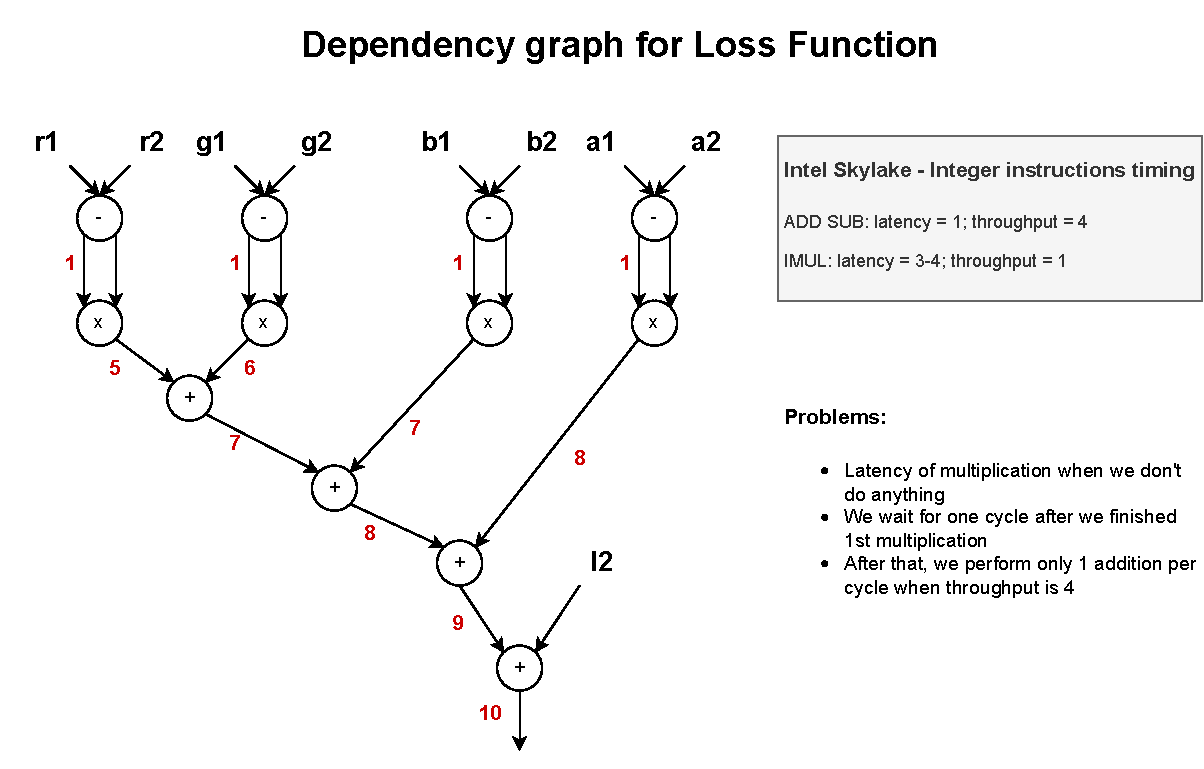
\includegraphics[scale=0.4]{DependencyGraph.pdf}
  \caption{Dependency graph of the $\ell^2$-loss function between two pixels, considering Intel Skylake microarchitecture. Channels {$r_{1}, r_{2}, g_{1}, g_{2}, ...$} correspond to the respective pixel channels.\label{dg}}
\end{figure}

To optimize the algorithm, let us determine the ideal unrolling factor that can effectively address these limitations. Within the algorithm, the number of additions outweighs the number of multiplications by a factor of two. Furthermore, the throughput of additions surpasses that of multiplications by a factor of four. Consequently, under optimal circumstances, it becomes feasible to parallelize slightly over half of all multiplications. Considering this, an unroll factor of 4 should suffice since it allows for parallelization of half of the multiplications. Specifically, for the first set of pixel pairs, the multiplication of differences can be executed in parallel with the subtractions of RGBA channel values from the subsequent 3 pairs. Similarly, for the final pixel pair, the multiplication can occur concurrently with the final additions. This assertion can be substantiated by examining the dependency graph provided in Fig.~\ref{unroll}. By employing this unrolling technique, we successfully minimized the number of cycles required per pixel to a mere 5.25. This value is only slightly larger than the best possible scenario for this algorithm. It serves as a favorable compromise since higher unrolling factors lead to increased code complexity and potential memory-related challenges arising from a larger number of accumulators.

\begin{figure}[htbp]
\centering
  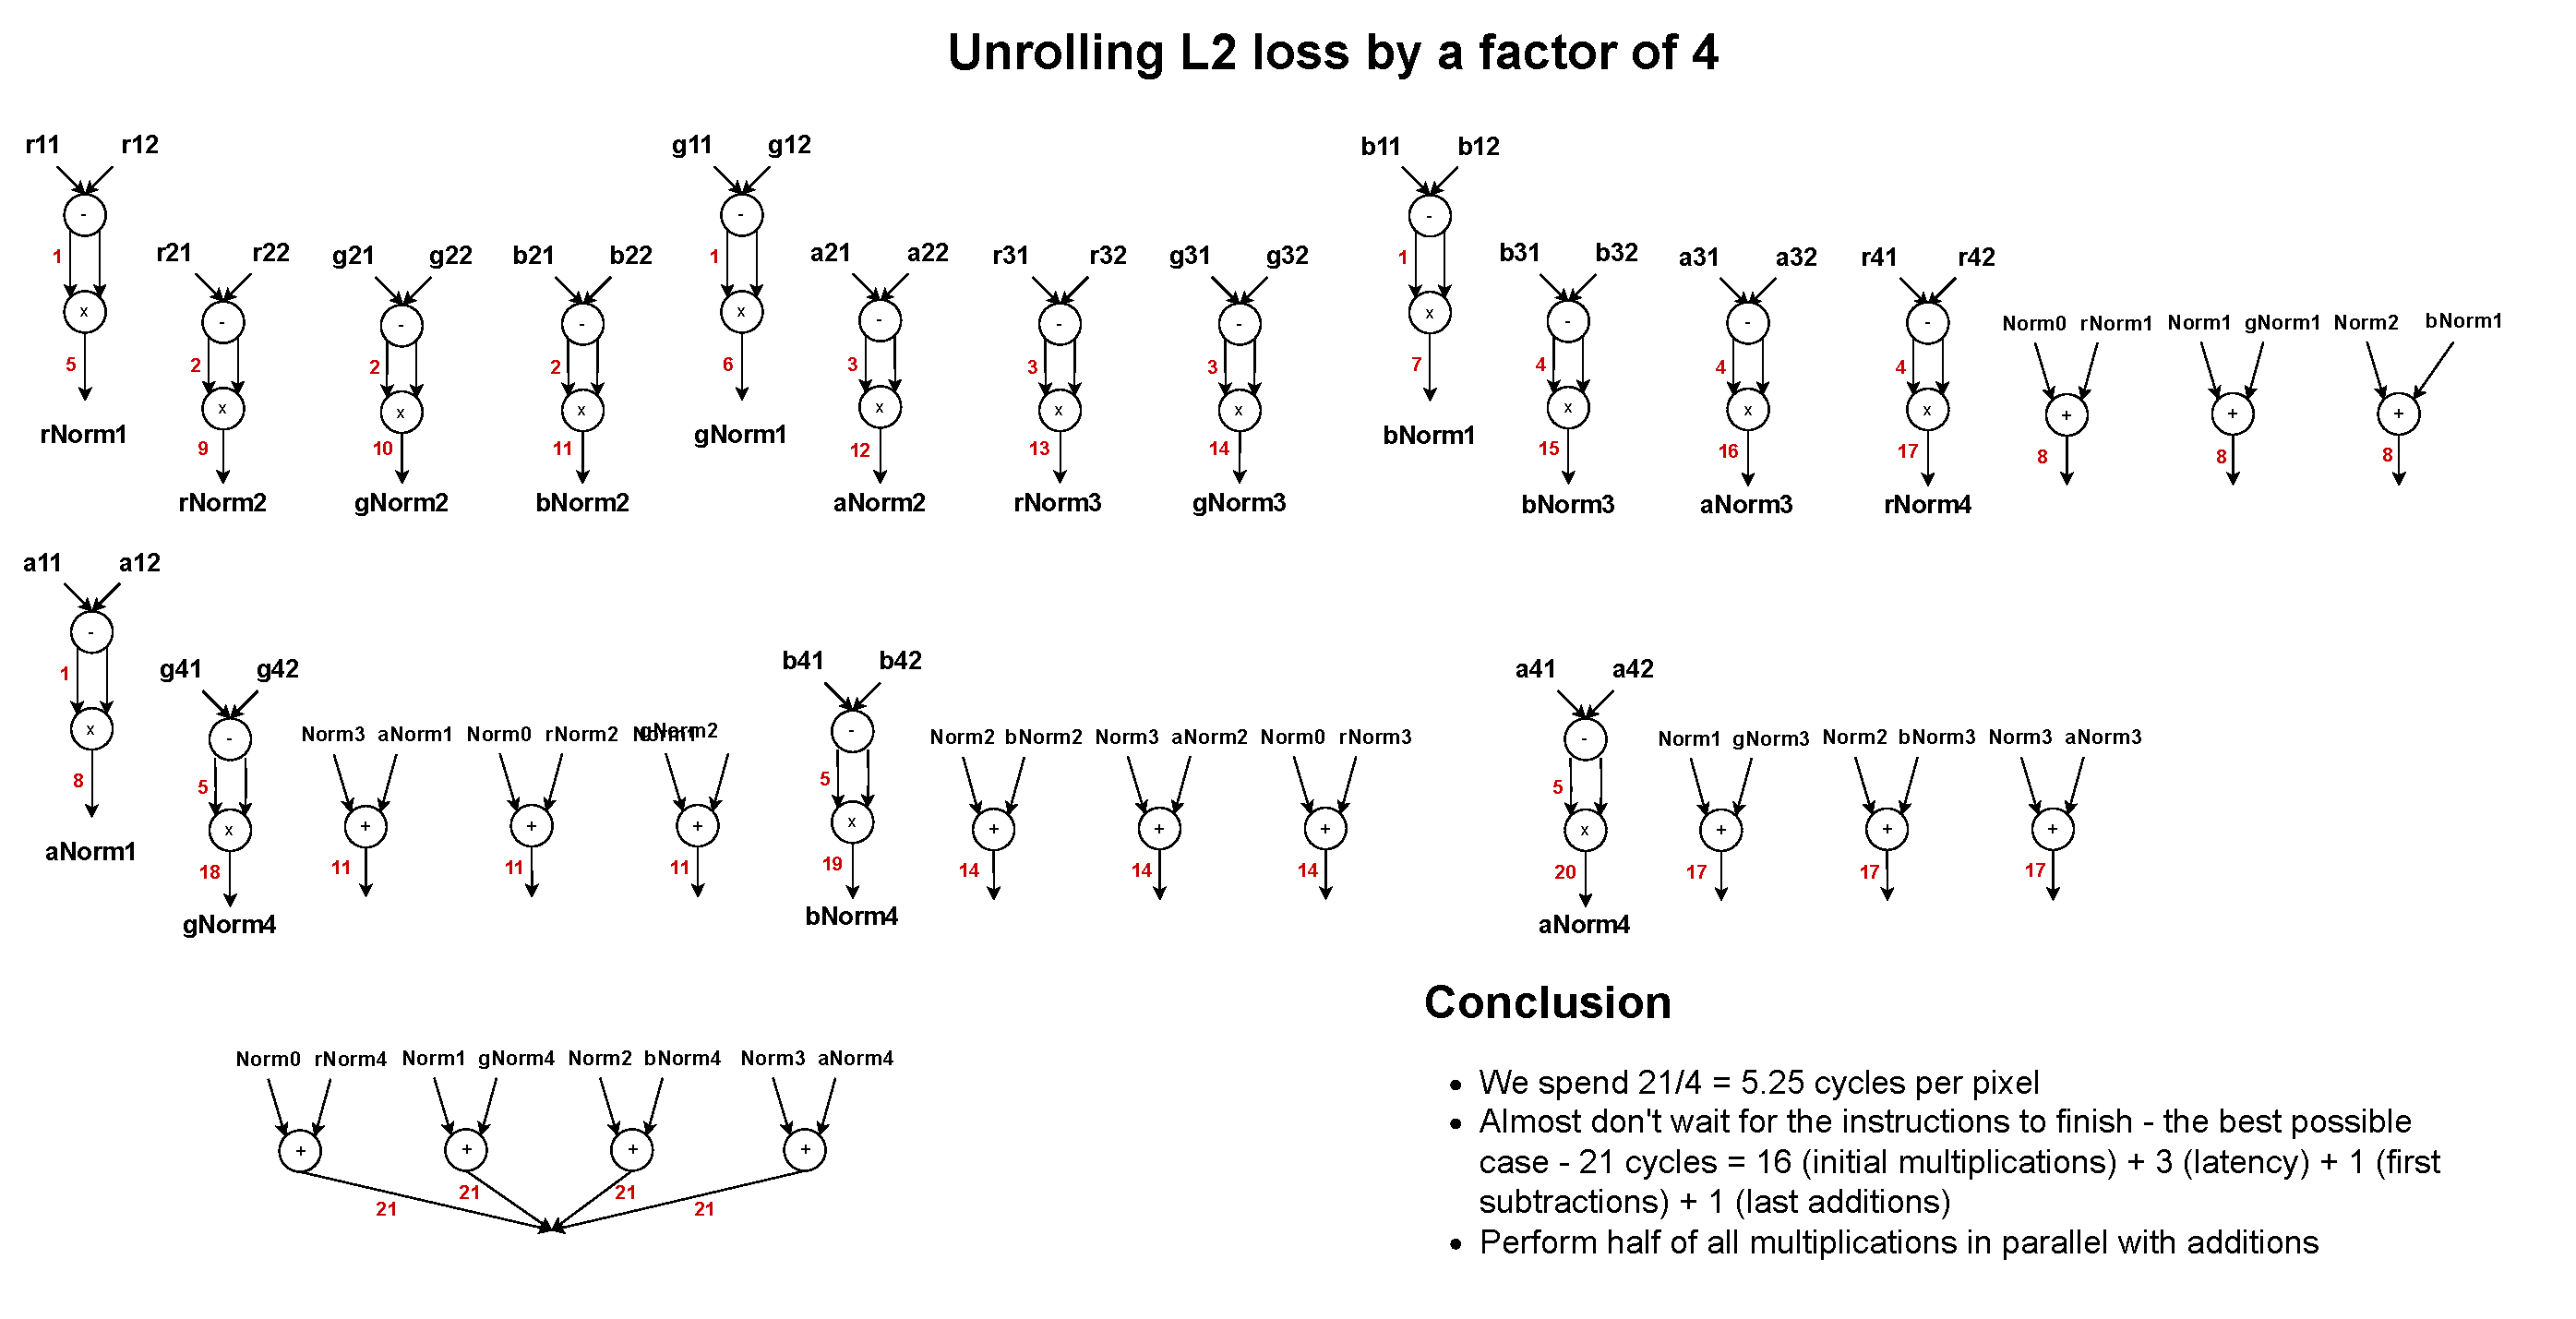
\includegraphics[scale=0.18]{Unrolling.pdf}
  \caption{Dependency graph of the $\ell^2$-loss function between two pixels with an unroll factor of 4, considering Intel Skylake microarchitecture.\label{unroll}}
\end{figure}

\mypar{Locality}

Understanding the temporal and spatial locality of memory access patterns is a crucial step in improving performance and efficiency by reducing the number of cache misses outside of the last level cache (LLC). We perform a temporal and spatial locality analysis of (1) selecting a new block and (2) performing the minimum cut.

\textit{(1) Selecting a Block.}

Recall that selecting a block consists of iterating over every potential source block in $S_b$, computing its $\ell ^2$-norm with respect to the overlap region in the output texture, and randomly sampling a block within a threshold of the lowest $\ell ^2$-norm. In our baseline implementation, we created a function called \inline{ComputeOverlap} whose sole purpose was to compute the $\ell ^2$-norm between the overlap region of the output texture and the overlap region of an individual source block. A single call to this function exhibits no temporal locality because each pixel in the output and input overlap regions is accessed exactly once. However, because our images are stored as two-dimensional arrays of packed 1-byte wide red, green, blue, and alpha channels, this function exhibits spatial locality, since pixels of the same row are stored contiguously in memory. In the baseline implementation we already took advantage of the spatial locality since we iterate through the overlap region row-by-row. Therefore, because the CPU reads contiguous cache blocks into the L1 and L2 caches, for a cache block size of $B$ we will have on average 1 compulsory cache miss to $B-1$ cache hits.

We then implemented selecting a block by calling the \inline{ComputeOverlap} function once for each potential source block in $S_b$. Although this approach results in readable and practical code, it leads to an enourmous amount of temporal locality. Firstly, each call to the \inline{ComputeOverlap} function iterates over every pixel of the the overlap region in the output texture, and so the overlap region in the output texture is read $|S_b|$ times. Secondly, although each call to the \inline{ComputeOverlap} function iterates over the overlap region of a different source block, consecutive source blocks often differ by a one-pixel-shift to the right, and hence their overlap regions admit a considerable amount of the same pixels. Non-consecutive source blocks that differ by horizontal or vertical shifts similarly admit overlap regions that share a substantial number of pixels.

TODO create diagrams illustrating the temporal locality.

We can address the temporal locality of iterating over the overlap region in the output texture $|S_b|$ times with a loop reordering. The baseline implementation calls the \inline{ComputeOverlap} function once for each potential source block in $S_b$, which gives us the following pseudo code:

\begin{lstlisting}[style=cppstyle]
  for i = 0 to maxBlockY - 1
    for j = 0 to maxBlockX - 1
      for k = 0 to overlapHeight - 1
        for l = 0 to overlapWidth - 1
          // Compute the l2 norm
\end{lstlisting}

Here the two inner loops iterate over the pixels of the overlap region and the outer two loops iterate over every potential source block. By reordering the inner and outer two loops, we can iterate over the pixels of the overlap region exactly once:

\begin{lstlisting}[style=cppstyle]
  for k = 0 to overlapHeight - 1
    for l = 0 to overlapWidth - 1
      for i = 0 to maxBlockY - 1
        for j = 0 to maxBlockX - 1
          // Compute the l2 norm
\end{lstlisting}

This loop reordering further allows us to block both iterating over the pixels of the overlap region as well as block iterating over pixels of the source texture, as we will discuss in the blocking subsection.

\textit{(2) Performing the Minimum Cut}

\mypar{Blocking} 

\mypar{Vectorization} When utilizing SIMD (Single Instruction, Multiple Data) vectorization, there are several considerations to keep in mind to maximize performance and efficiency: \\ 
\textit{Data alignment}: SIMD operations typically require data to be aligned on specific boundaries. We ensure that data is aligned by using \texttt{malloc}, which is guaranteed to be properly aligned for objects of any type. Maximum alignment size of \texttt{malloc} is determined by \texttt{max\_align\_t} which usually equals to size of \texttt{long double} (16 bytes). Maximum alignment will influence vector width selection.  \\
\textit{Data dependency}: Minimizing data dependencies within vectorized code is crucial for enabling parallel execution and fully utilizing SIMD capabilities. To achieve this, we apply insights discussed in the loop unrolling section, reducing idle CPU time. \\
\textit{Vector width}: In our case, we represent each pixel value as a 16-bit value with four components, each occupying one byte. To perform operations correctly, we load 16 8-bit values into a 128-bit integer variable and convert it into a 256-bit variable of 16-bit integers. This approach prevents overflow during multiplication and addition and maximizes performance by utilizing the available memory in the vector.\\
The majority of our vectorization efforts are dedicated to computing the $\ell^2$-loss function, as it is the most computationally expensive operation in our code. By optimizing this function, we can achieve significant performance improvements. \\
Through our experiments, we found that the "madd" (multiply-add) function is well-suited for our specific purpose of calculating the norm and performing horizontal component addition.
Furthermore, to mitigate data dependencies, we employed a loop unroll with a factor of x2 of the vector width. This approach allowed us to effectively reorder operations and minimize periods of idle CPU time. 

\section{Experimental Results}\label{sec:exp}

Here you evaluate your work using experiments. You start again with a
very short summary of the section. The typical structure follows.

\mypar{Experimental setup} Specify the platform (processor, frequency, cache sizes)
as well as the compiler, version, and flags used. I strongly recommend that you play with optimization flags and consider also icc for additional potential speedup.

Then explain what input you used and what range of sizes. The idea is to give enough information so the experiments are reproducible by somebody else on his or her code.

\mypar{Results}
Next divide the experiments into classes, one paragraph for each. In the simplest case you have one plot that has the size on the x-axis and the performance on the y-axis. The plot will contain several lines, one for each relevant code version. Discuss the plot and extract the overall performance gain from baseline to best code. Also state the percentage of peak performance for the best code. Note that the peak may change depending on the situation. For example, if you only do additions it would be 12 Gflop/s
on one core with 3 Ghz and SSE and single precision floating point.

Do not put two performance lines into the same plot if the operations count changed significantly (that's apples and oranges). In that case first perform the optimizations that reduce op count and report the runtime gain in a plot. Then continue to optimize the best version and show performance plots.

{\bf You should}
\begin{itemize}
\item Follow to a reasonable extent the guide to benchmarking presented in class, in particular
\item very readable, attractive plots (do 1 column, not 2 column plots
for this class), proper readable font size. An example is below (of course you can have a different style),
\item every plot answers a question, which you pose and extract the
answer from the plot in its discussion
\end{itemize}
Every plot should be referenced and discussed (what does it show, which statements do
you extract).

\section{Conclusions}

Here you need to briefly summarize what you did and why this is
important. {\em Do not take the abstract} and put it in the past
tense. Remember, now the reader has (hopefully) read the paper, so it
is a very different situation from the abstract. Try to highlight
important results and say the things you really want to get across
(e.g., the results show that we are within 2x of the optimal performance ...
Even though we only considered the DFT, our optimization
techniques should be also applicable ....) You can also formulate next
steps if you want. Be brief.

\section{Further comments}

Here we provide some further tips.

\mypar{Further general guidelines}

\begin{itemize}
\item For short papers, to save space, I use paragraph titles instead of
subsections, as shown in the introduction.

\item It is generally a good idea to break sections into such smaller
units for readability and since it helps you to (visually) structure the story.

\item The above section titles should be adapted to more precisely
reflect what you do.

\item Each section should be started with a very
short summary of what the reader can expect in this section. Nothing
more awkward as when the story starts and one does not know what the
direction is or the goal.

\item Do not use subsubsections.

\item Make sure you define every acronym you use, no matter how
convinced you are the reader knows it.

\item Always spell-check before you submit.

\item Be picky. When writing a paper you should always strive for 
high quality. Many people may read it and the quality makes a big difference.
In this class, the quality contributes to the grade.

\item Books helping you to write better: \cite{Higham:98} and \cite{Strunk:00}.
\end{itemize}

\mypar{Graphics} For plots that are not images {\em never} generate (even as intermediate step)
jpeg, gif, bmp, tif. Use eps, which means encapsulate postscript, or pdf. This way it is
scalable since it is a vector graphic description of your graph. E.g.,
from Matlab, you can export to eps or pdf.

Fig.~\ref{fftperf} is an example plot that I used in a lecture. Note that the fontsize in the plot should not be any smaller. On the other hand it is also a good rule that the font size in the plot is not larger than the one in the caption (otherwise it looks ugly).

\begin{figure}\centering
  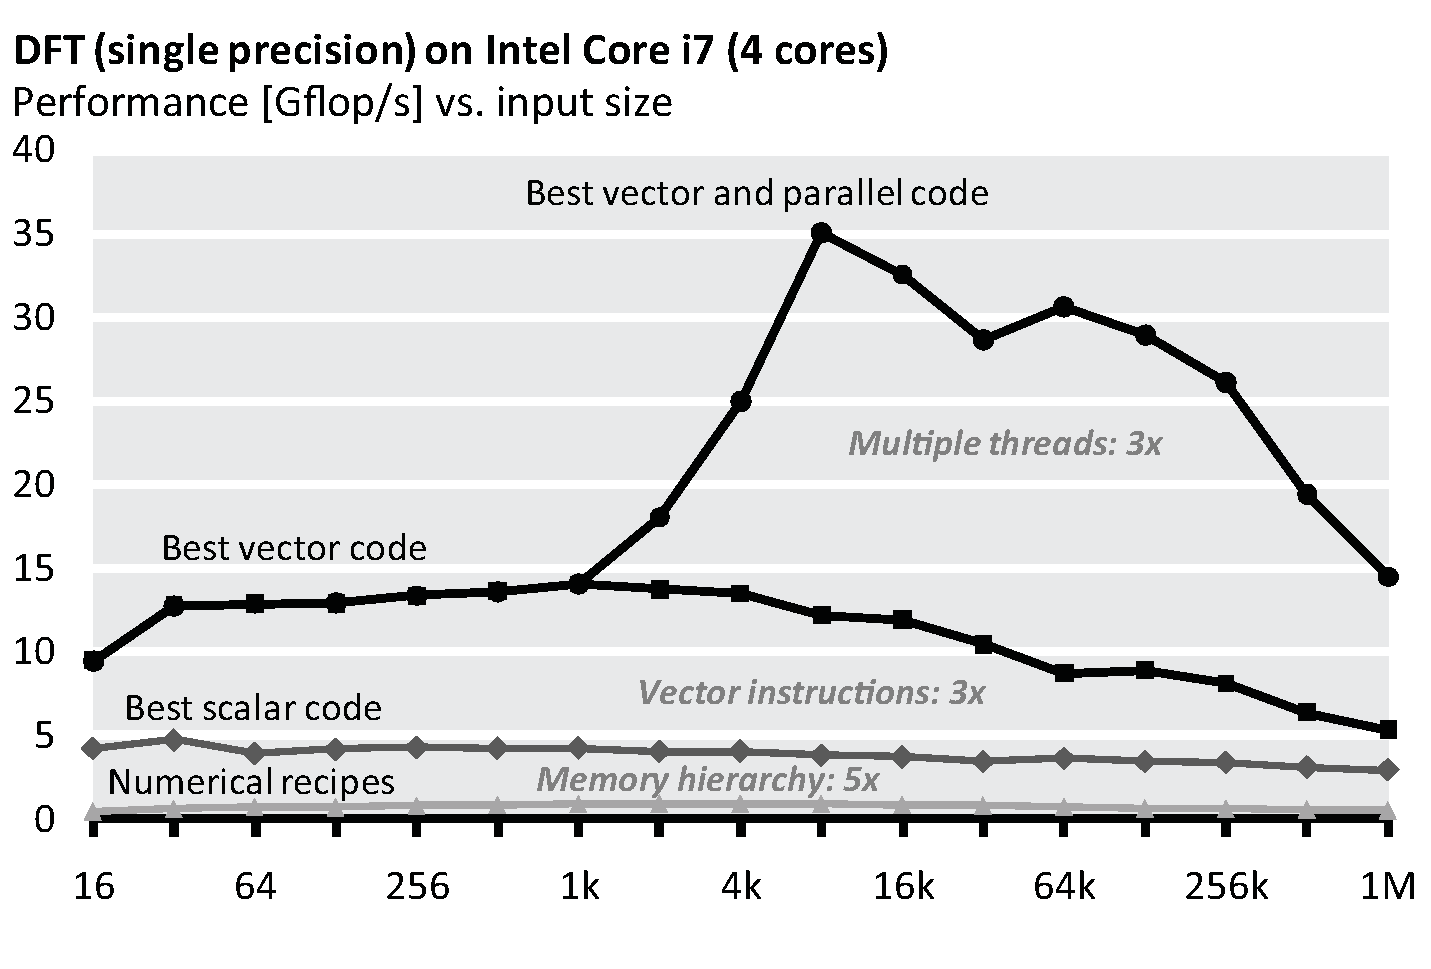
\includegraphics[scale=0.33]{dft-performance.pdf}
  \caption{Performance of four single-precision implementations of the
  discrete Fourier transform. The operations count is roughly the
  same. {\em The labels in this plot are about the smallest you should go.}
  \label{fftperf}}
\end{figure}

\bigskip
{\bf Up to here you have 8 pages.}

\section{Contributions of Team Members (Mandatory)}

In this mandatory section (which is not included in the 8 pages limit) each team member should very briefly (telegram style is welcome) explain what she/he did for the project. I imagine this section to be between one column and one page (absolute maximum).

Include only 
\begin{itemize}
	\item What relates to optimizing your chosen algorithm / application. This means writing actual code for optimization or for analysis.
	\item What you did before the submission of the presentation.
\end{itemize}
Do not include
\begin{itemize}
	\item Work on infrastructure and testing.
	\item Work done after the presentation took place.
\end{itemize}

Example and structure follows.

\mypar{Marylin} Focused on non-SIMD optimization for the variant 2 of the algorithm. Cache optimization, basic block optimizations, small generator for the innermost kernel (Section 3.2). Roofline plot. Worked with Cary and Jane on the SIMD optimization of variant 1, in particular implemented the bit-masking trick discussed.

\mypar{Cary} ...

\mypar{Gregory} ...

\mypar{Jane} ...

% References should be produced using the bibtex program from suitable
% BiBTeX files (here: bibl_conf). The IEEEbib.bst bibliography
% style file from IEEE produces unsorted bibliography list.
% -------------------------------------------------------------------------
\bibliographystyle{IEEEbib}
\bibliography{bibl_conf}

\end{document}
